
The core calculus of NomosUC is based on \emph{binary session types}~\cite{caires2010session}:
a type discipline for communication-centric programming derived from a Curry-Howard interpretation
of intuitionistic linear logic~\cite{girard1987linear}.
Under this correspondence, a process term $P$ is assigned to
a logical judgment of the form $A_1, \ldots A_n \vdash C$ and each antecedent as well as the succedent is
labeled with a \emph{channel} to obtain
\[
x_1 : A_1, \ldots, x_n : A_n \vdash P :: (z : C)
\]
The resulting judgment states that process $P$ \emph{provides} a service
of session type $C$ along channel $z$, \emph{using} the services of session
types $A_1, \ldots, A_n$ provided along channels $x_1, \ldots, x_n$ respectively.
We mandate all channel names to be distinct for the judgment
to be \emph{well-formed}.
The linear antecedents are often abbreviated to $\D$.

Formally, the typing judgment for processes in NomosUC is written as
$\Sg \semi k \semi \Tokens \semi \Psi \semi \D \entailpot{q}{q'} P :: (x : A)$.
$\Sg$ denotes the signature containing type and process definitions and $k$
denotes the security parameter.
Both these quantities are globally known and fixed, therefore we omit them from
most typing rules for brevity.
$\Tokens$ describes the total and current ($=$ received - sent) import tokens
of each type stored in the process (explained more in Section~\ref{sec:import}).
$\Psi$ represents the functional data structures and $\D$ collects the
session-typed channels along with an optional \emph{write token} $\wt$
(to resolve non-determinism in the semantics) used by the process.
Intuitively, the process sending a message \emph{must possess} the write
token which is then transferred to the receiver along with the write token.
Globally, the process owning the write token is activated to take the
next execution step.
Finally, $P$ is the process expression that is currently being executed and
the process offers channe $x$ of type $A$.
Similar to import tokens, the natural number annotations $q$ and $q'$ on the turnstile
denote the total and current potential stored in the process.
We will gradually explain each component of the language, initiating
with the basic system of session types.
For simplicity of exposition, we will display the yet unexplained
parts of the system in blue.

The operational semantics for session-typed programs are formalized as a
system of \emph{multiset rewriting rules}~\cite{cervesato2009relating}.
These rules consist of semantic objects $\proc{c}{P}$ and $\msg{c}{M}$ describing
process $P$ (or message $M$) providing service along channel $c$.
Remarkably, in this formulation, a message is just a particular form of process,
thereby not requiring any special rules for typing; it can be typed just as processes.
Since we track computational cost as well in NomosUC, we extend the semantic objects
to $\proc{c}{w, P}$ and $\msg{c}{w, P}$ where work counter $w$ stores the work performed
(number of computational steps executed) by process $P$ (resp. message $M$).

\subsection{Session Type Constructors}
\label{subsec:constructors}

The Curry-Howard correspondence gives each linear logic connective an
interpretation as a session type.
We follow a detailed description of each of these session type constructors,
but restricted to a subset that are sufficient for the applications of NomosUC.

\paragraph*{\textbf{Choice Operators}}
The internal choice $\ichoice{\ell : A_\ell}_{\ell \in L}$ constructor
is an $n$-ary labeled generalization of the additive disjunction $A \oplus B$.
A process that provides $x : \ichoice{\ell : A_\ell}_{\ell \in L}$ can send
any label $k \in L$ along $x$ and then continue by providing $x : A_k$. The
corresponding process is written as $(\esendl{x}{k} \semi P)$, where
$P$ is the continuation that provides $A_k$.
On the other end of the channel, the client branches on the label received along $x$.
The provider and client are typed according to the following $\oplus R$ and $\oplus L$
rules respectively.
\begin{mathpar}
  \infer[{\oplus}R]
  {\B{\Tokens \semi \Psi} \semi \wt, \D \entailpot{\B{q}}{\B{q'}} (\esendl{x}{k} \semi P) ::
    (x : \ichoice{\ell : A_\ell}_{\ell \in L})}
  {(k \in L) \qquad \B{\Tokens \semi \Psi} \semi \D \entailpot{\B{q}}{\B{q'}} P :: (x : A_k)}
\and
  \infer[{\oplus}L]
  {\B{\Tokens \semi \Psi} \semi \D, (x : \ichoice{\ell : A_\ell}_{\ell \in L})
    \entailpot{\B{q}}{\B{q'}} \ecase{x}{\ell}{Q_\ell}_{\ell \in L} :: (z : C)}
  {(\forall \ell \in L) \qquad \B{\Tokens \semi \Psi} \semi \wt, \D, (x : A_\ell)
    \entailpot{\B{q}}{\B{q'}} Q_\ell :: (z : C)}
\end{mathpar}
Additionally, the provider should possess the write token to be able to send the
label $k$. Dually, the client receives the write token with the label to continue
execution.

Operationally, since communication is asynchronous, the process
$(\esendl{c}{k} \semi P)$ sends a message $k$
along $c$ and continues as $P$ without waiting for it to be received.
As a technical device to ensure that consecutive messages on a
channel arrive in order, the sender also creates a fresh continuation
channel $c'$ so that the message $k$ is actually represented as
$(\esendl{c}{k} \semi \fwd{c}{c'})$ (read: send $k$ along $c$ and
continue as $c'$). The provider substitutes $c'$ for $c$ enforcing
that the next message is sent on $c'$.
The work counter of the process remains unaltered, and the new message
is created with work $0$.
\begin{tabbing}
$(\oplus S) : \proc{c}{w, \esendl{c}{k} \semi P} \step \proc{c'}{w, [c'/c]P},
\msg{c}{0, \esendl{c}{k} \semi \fwd{c}{c'}}$
\end{tabbing}
When the message $k$ is received along $c$, the client selects branch
$k$ and also substitutes the continuation channel $c'$ for $c$, thereby
ensuring that it receives the next message on $c'$. This implicit
substitution of the continuation channel ensures the ordering of the
messages.
The client process also collects the work performed by the message, if
there is any.
\begin{tabbing}
$(\oplus C) :$ \= $\msg{c}{w, \esendl{c}{k} \semi \fwd{c}{c'}},
\proc{d}{w', \ecase{c}{\ell}{Q_\ell}}
\step \proc{d}{w+w',[c'/c]Q_k}$
\end{tabbing}

The dual of internal choice is \emph{external choice} $\echoice{\ell :
A_\ell}_{\ell \in L}$, the $n$-ary labeled generalization of the
additive conjunction $A \with B$. This dual operator simply reverses
the role of the provider and client. The provider process of
$x : \echoice{\ell : A_\ell}_{\ell \in L}$ branches on receiving a label
using the expression $\ecase{x}{\ell}{Q_\ell}_{\ell \in L}$,
while the client sends one such label in $L$ using the expression $(\esendl{x}{k} \semi P)$.
% $k \in L$ (described in $\with R$), while the client sends this label
% (described in $\with L$).
% \begin{mathpar}
%   \footnotesize
%   \infer[\with R]
%   {\B{k \semi \Tokens \semi \Psi} \semi \D \entailpot{\B{q}}{\B{q'}} \ecase{x}{\ell}{P_\ell}_{\ell \in L} ::
%     (x : \echoice{\ell : A_\ell}_{\ell \in L})}
%   {(\forall \ell \in L) \qquad \B{k \semi \Tokens \semi \Psi} \semi \wt, \D
%     \entailpot{\B{q}}{\B{q'}} P_\ell :: (x : A_\ell)}
% \end{mathpar}
% \begin{mathpar}
%   \footnotesize
%   \infer[\with L]
%   {\B{k \semi \Tokens \semi \Psi} \semi \wt, \D, (x : \echoice{\ell : A_\ell}_{\ell \in L})
%     \entailpot{\B{q}}{\B{q'}} \esendl{x}{k} \semi Q :: (z : C)}
%   {\B{k \semi \Tokens \semi \Psi} \semi \D, (x : A_k) \entailpot{\B{q}}{\B{q'}} Q :: (z : C)}
% \end{mathpar}
Dual to internal choice, the client contains the write token which is
sent to the provider along with the label.
The operational semantics rules are also just the inverse of internal choice,
and therefore skipped for brevity.

\paragraph*{\textbf{Termination}}
The type $\one$, the multiplicative unit of linear logic, represents
termination of a process, which (due to linearity) is not allowed to use
any channels. A terminating process offering on $x : \one$ simply
closes channel $x$ while the client waits for this close message to arrive.
\begin{mathpar}
  \infer[{\one}R]
  {\B{k \semi \Tokens \semi \Psi} \semi \wt \entailpot{\B{q}}{\B{q'}} \eclose{x} :: (x : \one)}
  {\B{q = 0}}
  \and
  \infer[{\one}L]
  {\B{k \semi \Tokens \semi \Psi} \semi \D, (x : \one) \entailpot{\B{q}}{\B{q'}} (\ewait{x} \semi Q) :: (z : C)}
  {\B{k \semi \Tokens \semi \Psi} \semi \wt, \D \entailpot{\B{q}}{\B{q'}} Q :: (z : C)}
\end{mathpar}
Similar to internal choice, the closing process transfers the write
token to its waiting client along with the close message.
Additionally, the terminating process does not store
any potential since it cannot take any further execution steps
(explained more in Section~\ref{sec:import}).
% Operationally, the provider converts into a closing message
% with no continuation since the offered channel terminates.
% \begin{tabbing}
% $(\one S) : \proc{c}{\eclose{c}} \step \msg{c}{\eclose{c}}$ \\
% $(\one C) : \msg{c}{\eclose{c}}, \proc{d}{\ewait{c} \semi Q} \step
% \proc{d}{Q}$
% \end{tabbing}

% The provider receives the branching label $k$ sent by the provider. Both
% processes perform appropriate substitutions to ensure the order of messages
% sent and received is preserved.
% \[
% \begin{array}{lll}
% (\with S) & \proc{d}{\esendl{c}{k} \semi Q} \step \msg{c'}{\esendl{c}{k}
% \semi \fwd{c'}{c}}, \proc{d}{[c'/c]Q} & \fresh{c'} \\
% (\with C) & \proc{c}{\ecase{c}{\ell}{Q_\ell}_{\ell \in L}},
% \msg{c'}{\esendl{c}{k} \semi \fwd{c'}{c}} \step \proc{c'}{[c'/c]Q_k}
% \end{array}
% \]

\paragraph*{\textbf{Exchanging Functional Data}}
Communicating a \emph{value} of the functional fragment along a channel
is expressed at the type level by adding the following two session types.
\begin{center}
\begin{minipage}{0cm}
\begin{tabbing}
$A ::= \ldots \mid \tau \arrow A \mid \tau \product A$
\end{tabbing}
\end{minipage}
\end{center}
Here, $\tau$ describes a functional type, e.g. $\m{int}, \m{bool}, \tau \; \m{list}$, etc
(we assume the language contains standard functional types).
The type $\tau \arrow A$ prescribes receiving a value of type $\tau$
with continuation type $A$, while its dual $\tau \product A$ prescribes
sending a value of type $\tau$ with continuation $A$. The corresponding
typing rules for arrow ($\arrow R, \arrow L$) are given
below (rules for $\product$ are inverse).
\begin{mathpar}
  \infer[\arrow R]
  {\B{\Tokens} \semi \Psi \semi \D \entailpot{\B{q}}{\B{q'}}
  \erecvch{x}{v} \semi P :: (x : \tau \arrow A)}
  {\B{k \semi \Tokens} \semi \Psi, (v : \tau) \semi \wt, \D \entailpot{\B{q}}{\B{q'}}
  P :: (x : A)}
  %
  \and
  %
  \inferrule*[right = $\arrow L$]
  {\B{r' = p+q'} \qquad
  \B{\Psi \share (\Psi_1, \Psi_2)} \qquad
  \Psi_1 \exppot{\B{p}} M : \tau \\
  \B{k \semi \Tokens} \semi \Psi_2 \semi \D, (x : A) \entailpot{\B{q}}{\B{q'}}
  Q :: (z_k : C)}
  {\B{k \semi \Tokens} \semi \Psi \semi \wt, \D, (x : \tau \arrow A)
  \entailpot{\B{q}}{\B{r'}} \esendch{x}{M} \semi Q :: (z : C)}
\end{mathpar}
As indicated in the $\arrow R$ rule, receiving a value $y : \tau$ on a channel
$x : \tau \arrow A$ adds it to the functional context $\Psi$. On the
other hand, sending (value of) expression $M$ on channel $x : \tau \arrow A$
requires that $M$ has type $\tau$ (third premise).
The premises indicated in blue describe how potential is divided across
the functional and session-typed layers and will be described next.
Intuitively, the potential in functional context $\Psi$ is \emph{shared}
between $\Psi_1$ and $\Psi_2$ (second premise); $\Psi_1$ is used to type
$M$ while $\Psi_2$ is passed on to the continuation $Q$.

\subsection{Expressing ITMs With Session Types}
Despite the seemingly stuctured nature of execution in UC, the framework is meant to capture arbitrary connections, communication patterns, or configurations of ITMs. 
In this section we highlight a common pattern in UC that requires additional machinery to be express with session types.

The pattern emerges from the following code: a machine $P$ either writes to another machine $Q$ or is written to by $Q$. 
At first glance, it is a trivial scenario, but we encounter a problem trying to encode this with a single session type.
A example are machines $P$ and $Q$ which execute as follows:
\begin{itemize}
	\item An external machines flips a bit and activates either $P$ or $Q$.
	\item If $P$ is activated it writes to $Q$ and the execution terminates. 
	\item Otherwise, if $Q$ is activated, it writes a message to $P$, $P$ writes something back, and the execution terminates.
\end{itemize}
A single type between $P$ and $Q$ would have to allow either of the two parties to write on the channel, but session types require it to be statically known.

If we try to separate communication between $P$ and $Q$ into two uni-directional channel, we can express the session type for each of the channels:
\begin{center}
\parbox{0cm}{
\begin{tabbing}
$\m{PtoQ} = \ichoice{\mb{``one''}: int \tensor 1}$ \\
$\m{QtoP} = \echoice{\mb{``one''}: int \tensor \ichoice{\mb{``end''}: int \tensor 1}}$
\end{tabbing}}
\end{center}

This approach, however, poses another problem. 
Channels are only created by a process offering them, and a process can only offer a single channel.
Without adding any additional processes, $P$ must offer a channel to $Q$ and $Q$ offer one to $P$. 
Each of them becomes both a provider and a client to the other, and provider/client ambiguity is not allowed in Nomos. 
Logically, one process must have spawned the other, and such a cycle would be impossible to realize.

In order to capture this communication, and, in general, to break all possible cycles while still making meaningful use of session types, we propose a construction like Figure~\ref{fig:newpandq}.
We wrap each of $P$ and $Q$ in shell code, call them $S_P$ and $S_Q$, which spawn two dummy proceses to offer each of the channels of type \m{PtoQ} and \m{QtoP} to $P$ and $Q$.
The arrows within each shell represent the direction of communication rather than a provider-client relationship. 
In reality, any of the process can offer any of the channels as long as it doesn't result in a cycle.
\begin{figure}
	\begin{subfigure}{0.3\textwidth}
	\centering
	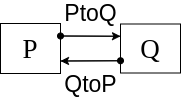
\includegraphics[scale=0.4]{figures/p_and_q.png}
	\caption{$P$ and $Q$ connected by two logical channels which are actually implemented by the figure on the right.}
	\label{fig:pandq}
	\end{subfigure}
	~ \ \ \ \ 
	\begin{subfigure}{0.6\textwidth}
	\centering
	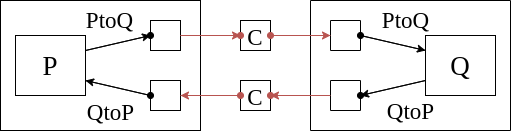
\includegraphics[scale=0.4]{figures/new_p_and_q.png}
	\caption{We can realize the left be intermediating communication with communicators. The direction of messages from $P$ to $Q$ still suggest a cycle but the communicator is provider (dot) to \emph{both} shell codes.}
	\label{fig:newpandq}
	\end{subfigure}
	\caption{Two ITM configurations. One possible with ITMs (left) and one realized in NomosUC (right). Arrows indicate direction of messages and the dot indicates the provider of the channel.}
\end{figure}
Communication between $S_1$ and $S_2$ along channels they each offer results in another cycle. 
Therefore, we break the cycle by intermediating their communication through a \emph{communicator}.
The communicator avoids cycles by offered a \emph{shared channel} rather than the typical linear channel.
We represent the communication in Figure~\ref{fig:newpandq} by Figure~\ref{fig:pandq} which abstracts away the implementation details of communicators and shell codes.

\paragraph*{\textbf{Shared Channels}}
\todo{Here I'm not too sure on whether this is enoug information or if it's correct.}
Linear channels are exclusive to the parent and child that are at their endpoints.
Balzer et al.~\cite{balzer2017manifest} proposed a \emph{shared} extension of session types which allows them to capture more natural programming scenarios where cyles naturally occurrs (ring network, dining philosophers, etc.).
Shared channels are still restricted to one provider but can be used by multiple clients to communicate with the provider. 
They introduce non-determinism that isn't present in UC where many clients can be attempting to communciate with the same provider, however, NomosUC borrows the write token from ILC to ensure activation and control are always with only on process at a time.

\paragraph*{\textbf{Communicators}}
Communicators act as channel buffers that two parties can use to communicate to each other.
The shared type of the communicators is given by 
\begin{center}
\parbox{0cm}{
\begin{tabbing}
$\m{comm[a]} = \up \echoice{$\=$\mb{SEND}: \m{a} \product \m \down \m{comm[a]},$\\
\>$\mb{RECV}: \ichoice{$\=$\mb{yes}: \m{a} \product \down \m{comm[a]},$\\
\>\>$\mb{no}: \down \m{comm[a]}}}$
\end{tabbing}}
\end{center}
The $\up$ and $\down$ operations around the session type indicate that it is \emph{shared}, and they denote a \emph{critical section} analogous to traditional concurrency controls like the mutex.
The type suggests that one party can send a message to the communicator, the communicator, buffers the message, and responds with it when asked to \m{RECV} is from a another process.

Communicators are parametric in a messages type \inline{a}.
Only channels in Nomos can be session typed, and  allowing channels to be sent over communicators enables flawed non-UC behavior.
Therefore, communicators are limited to buffering functionally typed messages.
This places extra functionality in the two spawned processes inside $S_1$ in Figure~\ref{fig:new_p_and_q}: the process must read functionally typed message and then send one on its session-typed channel and vice versa.

In general, mapping between functional and session-typed messages is achieved through a simple mapping between types and represents a systematic approach to intermediating communcation between $P$ and $Q$.
As we show in Section~\ref{sec:execuc}, we repeat this design pattern and rely on the creation of protocol-specific processes to conver functionally typed messages to session-typed messages.


\section{Syntax Sugar}
The machnery that we have introduced around NomosUC processes to achieve the expressiveness of ITMs is systematic in nature and can be statically defined given some protocol specification.
In this section we consider some syntatic sugar and automation around some parts of the NomosUC.

The first, and arguably most important, part of the 
